\documentclass[
BCOR 0.7cm,							% Bindekorrektur, bspw. 1 cm
11pt										% Schriftgroesse
]{scrbook}


\newif\ifpdf
\ifx\pdfoutput\undefined
	\pdffalse              	%normales LaTeX wird ausgef�hrt
\else
	\pdfoutput=1           
	\pdftrue               	%pdfLaTeX wird ausgef�hrt
\fi

\ifpdf
	%\usepackage{ae}        % Benutzen Sie nur
	%\usepackage{zefonts}  	% eines dieser Pakete
\else
	%%Normales LaTeX - keine speziellen Fontpackages notwendig
\fi

\ifpdf %%Einbindung von Grafiken mittels \includegraphics{datei}
	\usepackage[pdftex]{graphicx} %%Grafiken in pdfLaTeX
\else
	\usepackage[dvips]{graphicx} %%Grafiken und normales LaTeX
\fi


\ifpdf
	\pdfinfo
	{
    /Author (Manfred Kindl)                                
    /Title (Kalender)     
    /Subject (Kalender - Handbuch)
    /Keywords (CIS FH-Complete Kalender)	
  }
\else			
\fi

\usepackage{listings} \lstset{numbers=left, numberstyle=\tiny, numbersep=5pt}
\lstset{language=tex} 


\usepackage[pdftex,colorlinks=true,urlcolor=blue,linkcolor=blue]{hyperref}
\usepackage[ngerman]{babel}		%Deutsche Worttrennung	
\usepackage[T1]{fontenc}    % T1-Kodierung damit Umlaute richtig dargestellt werden
\usepackage[left]{eurosym}   %Paket f�rs Eurosymbol
\usepackage[latin9]{inputenc} % latin9 Encoding
\usepackage{makeidx} % Stichwortverzeichnis erstellen aus \index{} Eintr�gen
\usepackage{float}
\usepackage[small,bf]{caption}
\usepackage{fancyhdr} % Paket zur Manipulation von Kopf und Fusszeile
\usepackage{amssymb,amsmath}
\usepackage{color}

\addtokomafont{chapter}{\color[rgb]{0.0,0.376,0.584}}
\addtokomafont{section}{\color[rgb]{0.0,0.376,0.584}}
\addtokomafont{subsection}{\color[rgb]{0.0,0.376,0.584}}


\renewcommand{\rmdefault}{phv} % Arial
\renewcommand{\sfdefault}{phv} % Arial


\makeindex

\graphicspath{{../../../images/}}

\setlength{\tolerance}{2000}
\setlength{\parindent}{0pt}
\setlength{\parskip}{1ex plus 0.5ex minus 0.2ex}
\addtolength{\textheight}{2cm}
\addtolength{\headheight}{2pt}
\setlength{\captionmargin}{20pt}
\floatstyle{plain}
\floatname{example}{Example}

\newfloat{example}{hbtp}{loe}[chapter]
\floatplacement{figure}{hbtp}
\floatplacement{table}{htbp}

\newcommand{\dollar}{\char36}
\renewcommand{\labelitemi}{
\includegraphics[width=5pt]{blacksquare}}
\renewcommand{\labelitemii}{--}
%\renewcommand*{\chapterformat}{\textcolor{red}}

\newenvironment{info}[1]{
    \hspace{-10mm}
    \fbox{
        \begin{minipage}{1cm}
        
\includegraphics[width=1cm]{icon_info}
        \end{minipage}
        \begin{minipage}{14.5cm}
        #1
        \end{minipage}
    }
}

\newenvironment{achtung}[1]{
    \hspace{-10mm}
    \fbox{
        \begin{minipage}{1cm}
        
\includegraphics[width=1cm]{icon_achtung}
        \end{minipage}
        \begin{minipage}{14.5cm}
        #1
        \end{minipage}
    }
}

\newenvironment{halt}[1]{
    \hspace{-10mm}
    \fbox{
        \begin{minipage}{1cm}
        
\includegraphics[width=1cm]{icon_halt}
        \end{minipage}
        \begin{minipage}{14.5cm}
        #1
        \end{minipage}
    }
}

\newenvironment{idee}[1]{
    \hspace{-10mm}
    \fbox{
        \begin{minipage}{1cm}
        
\includegraphics[width=1cm]{icon_idee}
        \end{minipage}
        \begin{minipage}{14.5cm}
        #1
        \end{minipage}
    }
}


\setlength{\unitlength}{1mm}

\newenvironment{markier}[5]{
    
    \thicklines \put(#2,#3){\vector(#4,#5){5}} \thinlines
    \put(#2,#3){\circle*{5}}
    \put(#2,#3){\textcolor{black}{\circle{5}}\makebox(-10,0){\textcolor{white}{#1}}}


}


\hyphenation{gleich-zeitig para-meter}


\begin{document}

\ifpdf
	\DeclareGraphicsExtensions{.pdf,.jpg,.png}
\else
	\DeclareGraphicsExtensions{.eps}
\fi

\pagestyle{fancyplain}

% Titelseite einbinden
\begin{titlepage}
\begin{center}

\vspace*{40mm} \huge Handbuch\\
\vspace*{10mm}
\large \textsc{Kalenderschnittstellen}

\vfill 
\includegraphics[width=130mm]{fhcomplete}
	
\vfill \textsc{FH Technikum Wien}\\

Wien, \today
\end{center}
\end{titlepage}

\frontmatter					% Vorspann (z.B. r�mische Seitenzahlen)


\tableofcontents			% Inhaltsverzeichnis
%\listoftables				% Tabellenverzeichnis
%\addcontentsline{toc}{section}{Abbildungsverzeichnis}
%\listoffigures				% Abbildungsverzeichnis

%\chapter{Vorwort}


\mainmatter						% Hauptteil

%% Kapitel Anfang %%%%%%%%%%%%%%%%%%%%%%%%%%%%%%%%%%%%%%%%%%%%%%%%%

%% Kapitel Benotungstool Start
\chapter{Caldav}
\label{Caldav}
FH-Complete stellt eine Caldav Schnittstelle f�r LV-Plan Eintr�ge zur Verf�gung.\\
\\
Die Caldav Schnittstelle ist �ber folgende URL erreichbar:\\
\\
https://cis.technikum-wien.at/webdav/lvplan.php/calendars/<username>/LVPlan-<username>\\
\\
<username> ist durch den Loginnamen zu ersetzten.\\
\\
Die Caldav Schnittstelle liefert alle LV-Plan Eintr�ge des pers�nlichen LV-Plans des Benutzers in einem Zeitraum der letzten 2 Wochen und bis zu 6 Monate im vorraus.\\
\\
Es kann immer nur der eigene LV-Plan abboniert werden. Der LV-Plan anderer User kann derzeit nicht �ber Caldav abboniert werden.

\section{Kalender in Thunderbird Lightning Abbonieren}
\begin{enumerate}
	\item Datei->Neu->Kalender
	\item ''Im Netzwerk'' ausw�hlen
	\item Format: ''CalDAV'' ausw�hlen
	\item Adresse: siehe URL oben
	\item Name und Farbe vergeben
	\item Username und Passwort eingeben
\end{enumerate}


\begin{figure}[ht]
\begin{center}
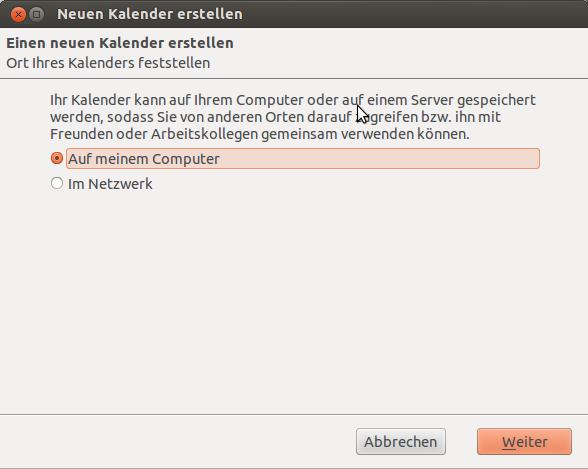
\includegraphics[width=1.0\textwidth]{CalDAVLightning1.png}
\end{center}
\end{figure}
\begin{figure}[ht]
\begin{center}
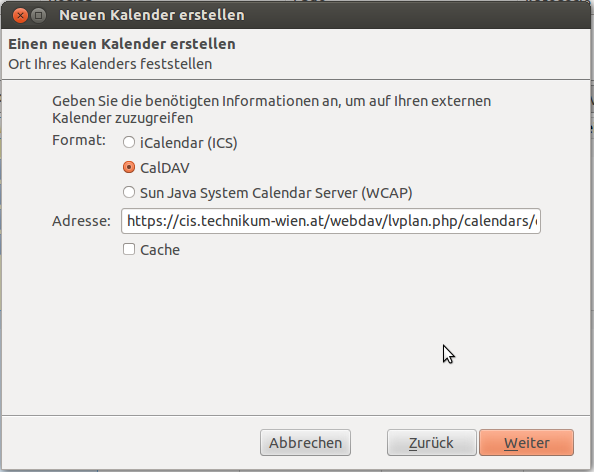
\includegraphics[width=1.0\textwidth]{CalDAVLightning2.png}
\end{center}
\end{figure}
\begin{figure}[ht]
\begin{center}
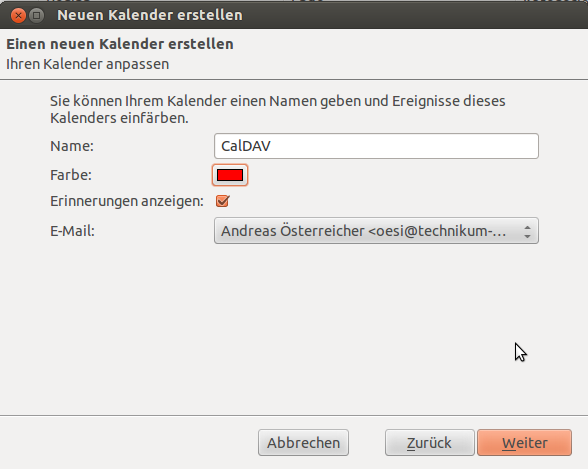
\includegraphics[width=1.0\textwidth]{CalDAVLightning3.png}
\end{center}
\end{figure}
\chapter{Freebusy}
\label{Freebusy}
Freebusy Informationen des pers�nlichen LV-Plans eines Users stehen unter foglender URL zur Verf�gung:
\\
https://cis.technikum-wien.at/cis/public/freebusy.php/<username>\\
\\
<username> ist durch den Loginnamen zu ersetzten.\\
\\
Die Freebusy URL enth�lt standardm��ig den pers�nlichen LV-Plan des Users.
Es gibt die M�glichkeit, diese Freebusy URL zu erweitern, um pers�nliche Kalender in diese URL mitaufzunehmen. (zB Horde Webmail, Google Kalender, DAViCal, etc)
\section{Zus�tzliche Freebusy URLs hinzuf�gen}
�ber den Punkt ''Neuen Eintrag hinzuf�gen'' k�nnen zus�tzliche Freebusy URLs hinzugef�gt werden.
Alle Eintr�ge werden zu einer gesammelten Freebusy URL vereint.

\begin{figure}[ht]
\begin{center}
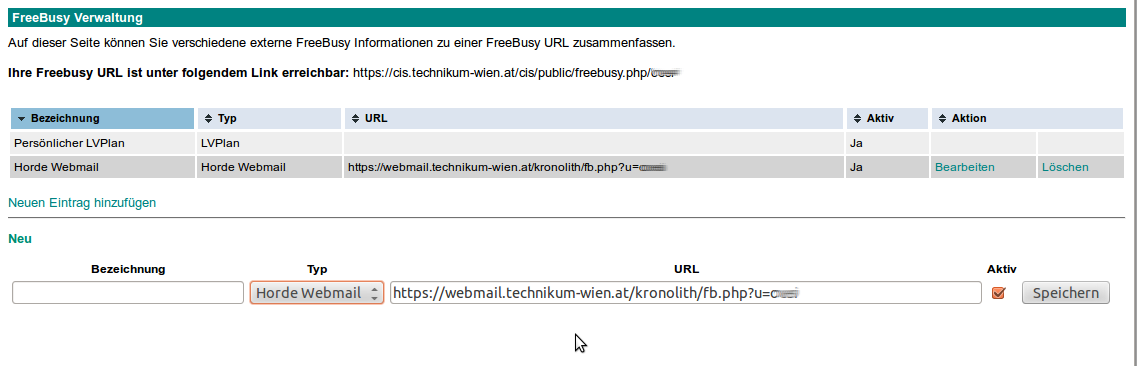
\includegraphics[width=1.0\textwidth]{freebusy_neu.png}
\end{center}
\caption{FreeBusy URL hinzuf�gen}\label{FreeBusy URL hinzuf�gen}
\end{figure}

\begin{enumerate}
	\item Bezeichnung: Freitext Bezeichnung der URL
	\item Typ: Anbieter der URL
	\item URL: Pfad zur FreeBusy URL die hinzugef�gt werden soll (wird in manchen F�llen bei der Auswahl des Typs vorgeschlagen)
	\item Aktiv: Dieses Hackerl muss gesetzt sein, damit die Eintr�ge in die FreeBusy URL aufgenommen werden
\end{enumerate}

Der pers�nliche LVPlan ist automatisch zur FreeBusy URL zugeordnet und kann nicht entfernt werden.
%% Kapitel Benotungstool Ende


%% Kapitel Ende   %%%%%%%%%%%%%%%%%%%%%%%%%%%%%%%%%%%%%%%%%%%%%%%%%


\appendix							% Beginn des Anhangs
%\chapter{Schluss}

\end{document}